\begin{figure}[htb]
	\centering
	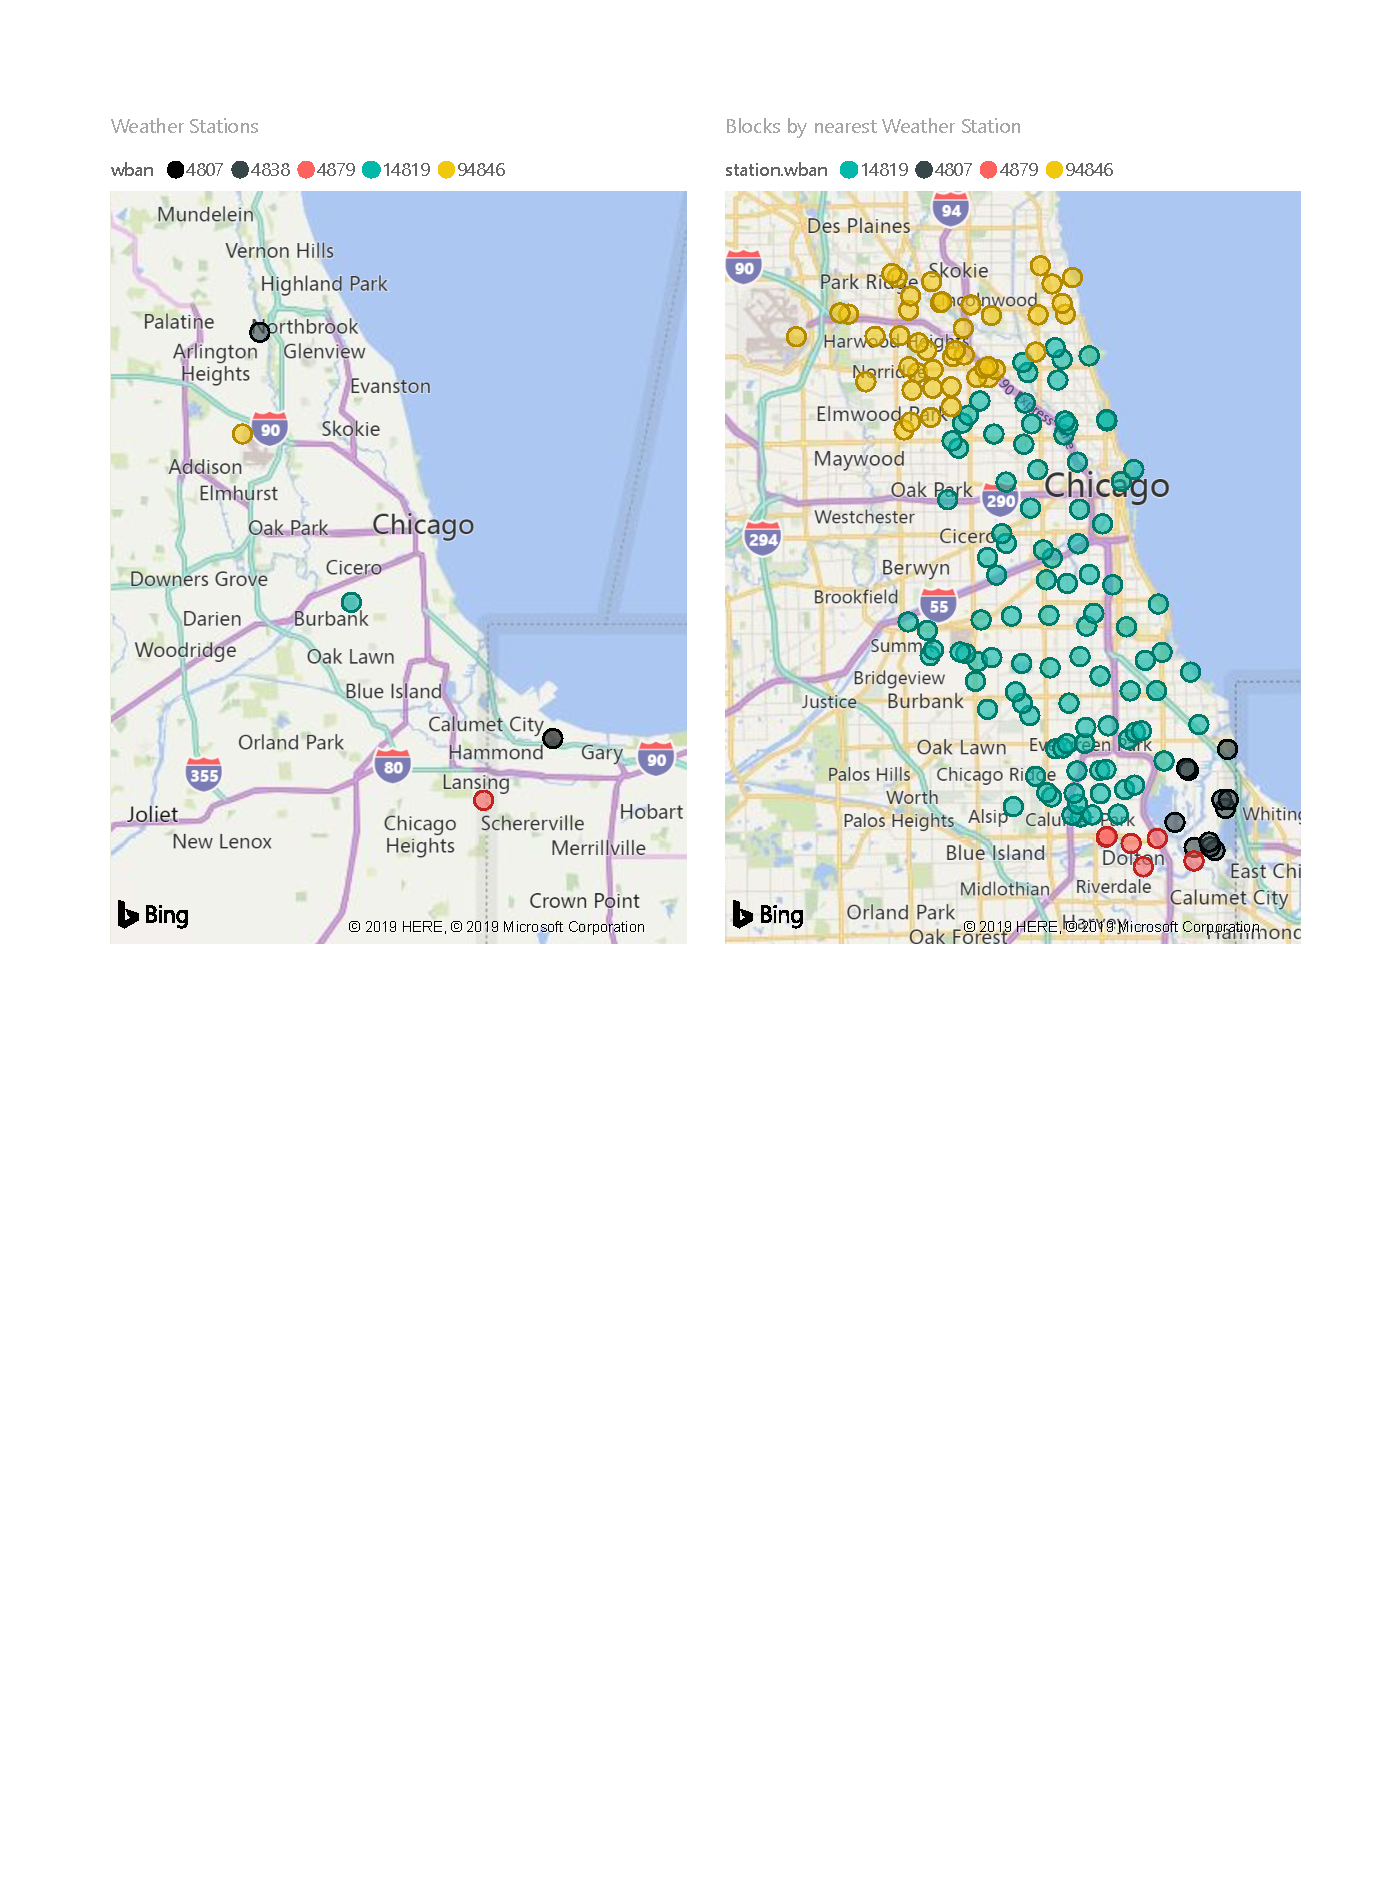
\includegraphics[width=0.4\columnwidth]{images/WeatherStations}
	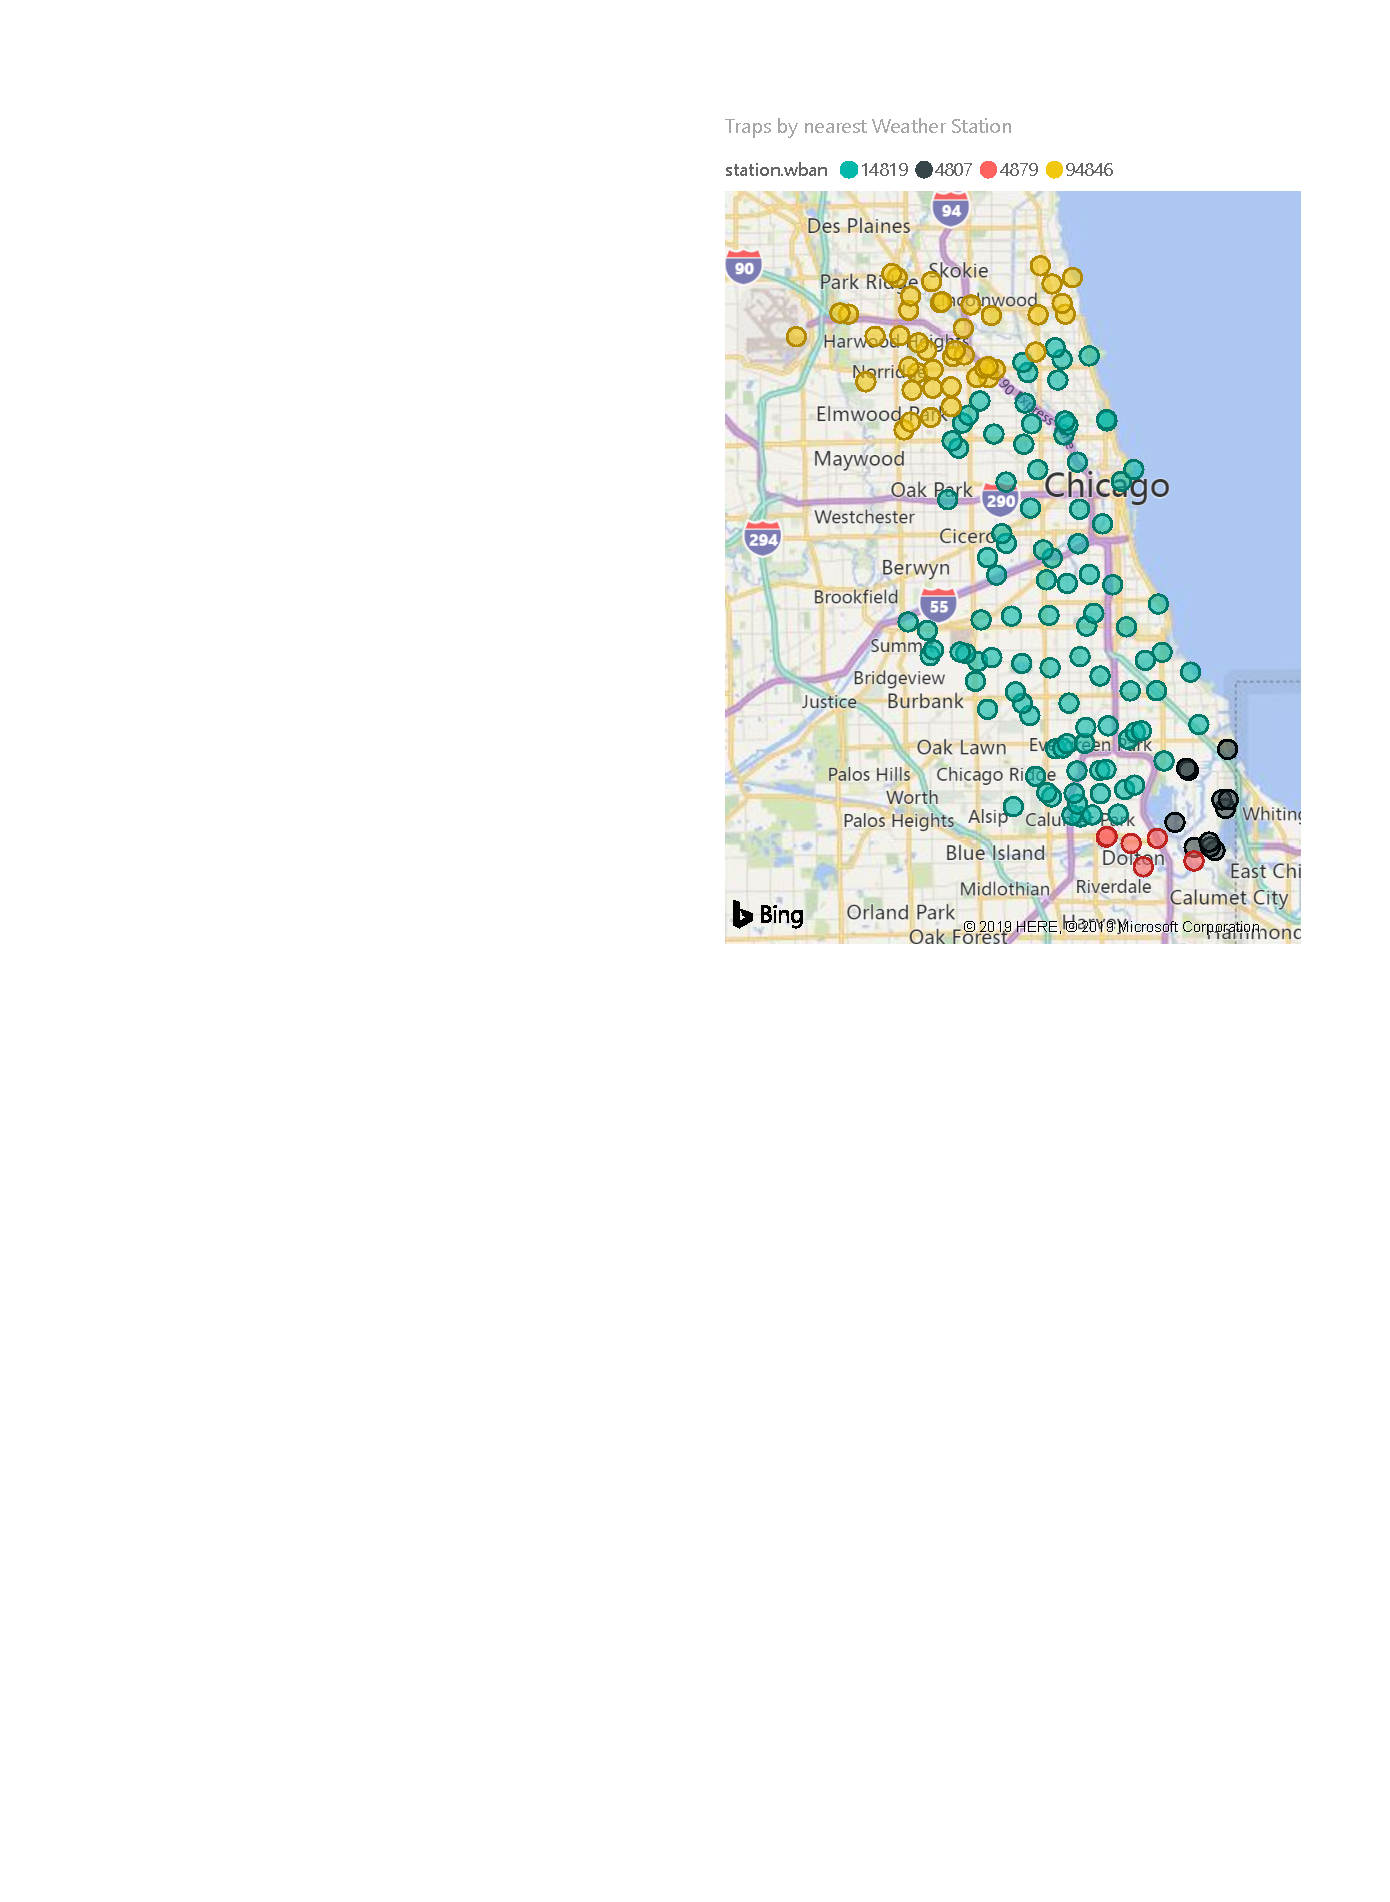
\includegraphics[width=0.4\columnwidth]{images/TrapsByNN}
	\caption{FIXME Visualizzazione dei 64 filtri convoluzionali appresi dal 
	layer \textbf{conv1} della rete ResNet-34. Il blu scuro rappresenta i 
	valori negativi, il verde quelli prossimi allo zero e il giallo quelli 
	positivi}
	\label{fig:weather-stations}
\end{figure}